% Schematic compensated barrier pulse and the resulting exchange response.
\begingroup
\definecolor{exchangePulseBlue}{HTML}{0072B2}
\definecolor{exchangePulseOrange}{HTML}{D55E00}
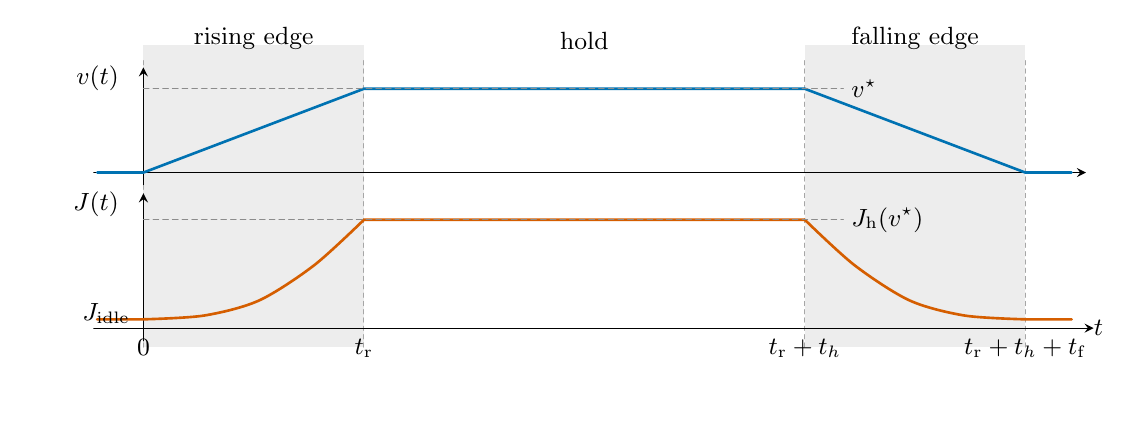
\begin{tikzpicture}[
 x=14mm,y=8mm,>=stealth,line cap=round,line join=round,
 every node/.style={font=\small,inner sep=1.5pt}
]
 \path[use as bounding box] (-1.05,-0.45) rectangle (8.85,5.35);

 % The two shaded intervals are the pulse edges.
 \fill[black!7] (0,0.28) rectangle (2,5.08);
 \fill[black!7] (6,0.28) rectangle (8,5.08);
 \node[anchor=south] at (1,4.93) {rising edge};
 \node[anchor=south] at (4,4.93) {hold};
 \node[anchor=south] at (7,4.93) {falling edge};

 % Shared switching times.
 \foreach \x in {0,2,6,8}{
  \draw[black!35,dash pattern=on 1.5pt off 1.5pt,line width=0.4pt]
       (\x,0.28)--(\x,4.88);
 }

 % Applied compensated-barrier coordinate v(t).
 \draw[->,line width=0.45pt] (-0.45,3.05)--(8.55,3.05);
 \draw[->,line width=0.45pt] (0,2.86)--(0,4.72);
 \node[anchor=east] at (-0.18,4.55) {$v(t)$};
 \draw[exchangePulseBlue,line width=0.95pt]
       (-0.42,3.05)--(0,3.05)--(2,4.38)--(6,4.38)--(8,3.05)--(8.42,3.05);
 \draw[black!45,dash pattern=on 2pt off 1.5pt,line width=0.4pt]
       (0,4.38)--(6.35,4.38);
 \node[anchor=west] at (6.38,4.38) {$v^\star$};

 % Exchange coupling J(t).  Curved edges emphasize J's nonlinear voltage response.
 \draw[->,line width=0.45pt] (-0.45,0.58)--(8.62,0.58);
 \draw[->,line width=0.45pt] (0,0.38)--(0,2.72);
 \node[anchor=east] at (-0.18,2.55) {$J(t)$};
 \draw[exchangePulseOrange,line width=0.95pt]
       (-0.42,0.72)--(0,0.72)
       plot[smooth] coordinates {(0,0.72) (0.55,0.78) (1.05,1.02) (1.55,1.58) (2,2.30)}
       --(6,2.30)
       plot[smooth] coordinates {(6,2.30) (6.45,1.58) (6.95,1.02) (7.45,0.78) (8,0.72)}
       --(8.42,0.72);
 \draw[black!45,dash pattern=on 2pt off 1.5pt,line width=0.4pt]
       (0,2.30)--(6.35,2.30);
 \node[anchor=west] at (6.38,2.30) {$J_{\mathrm h}(v^\star)$};
 \node[anchor=east] at (-0.08,0.82) {$J_{\mathrm{idle}}$};

 % Time labels.
 \node[anchor=north] at (0,0.48) {$0$};
 \node[anchor=north] at (2,0.48) {$t_{\mathrm r}$};
 \node[anchor=north] at (6,0.48) {$t_{\mathrm r}+t_h$};
 \node[anchor=north] at (8,0.48) {$t_{\mathrm r}+t_h+t_{\mathrm f}$};
 \node[anchor=west] at (8.58,0.58) {$t$};
\end{tikzpicture}
\endgroup
